The application is developed with use of both server-side and client-side programming. This chapter will therefore present both side of the programming but firstly the needed changes found in study II is described. Security considerations and implementation is described at the end of the chapter. The implemented application can be found on attached CD.

\section{Design Changes}

\begin{figure}[h]
  \centering
  \begin{minipage}[b]{0.45\textwidth}
    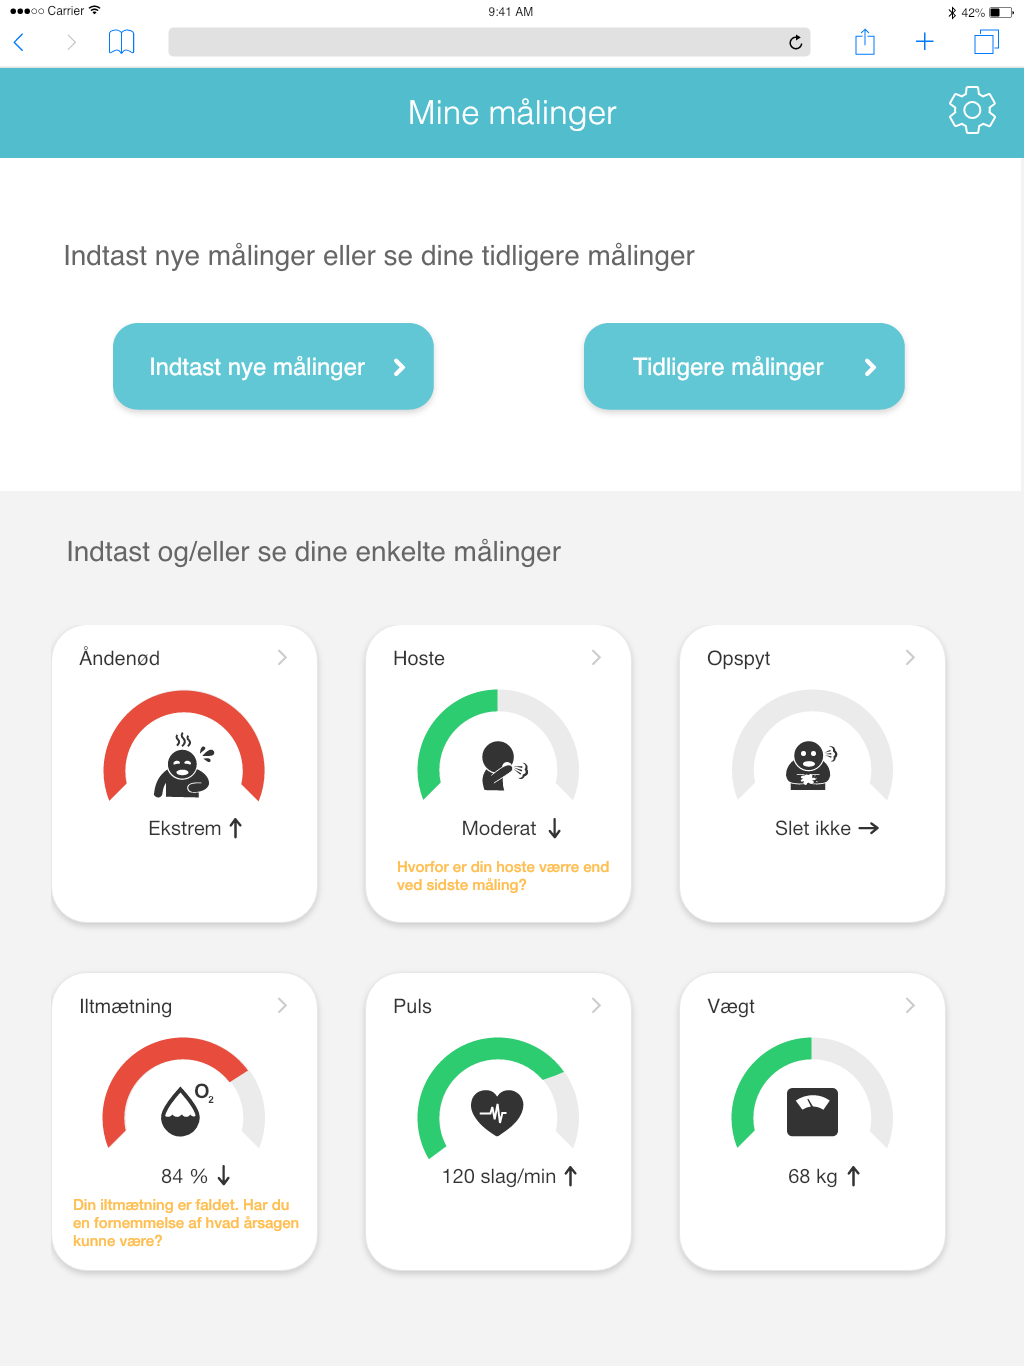
\includegraphics[width=\textwidth]{images/study2/Dashboard.png}
    \caption{Shows the dashboard used in study II.}
    \label{fig:db1st}
  \end{minipage}
  \hfill
  \begin{minipage}[b]{0.45\textwidth}
    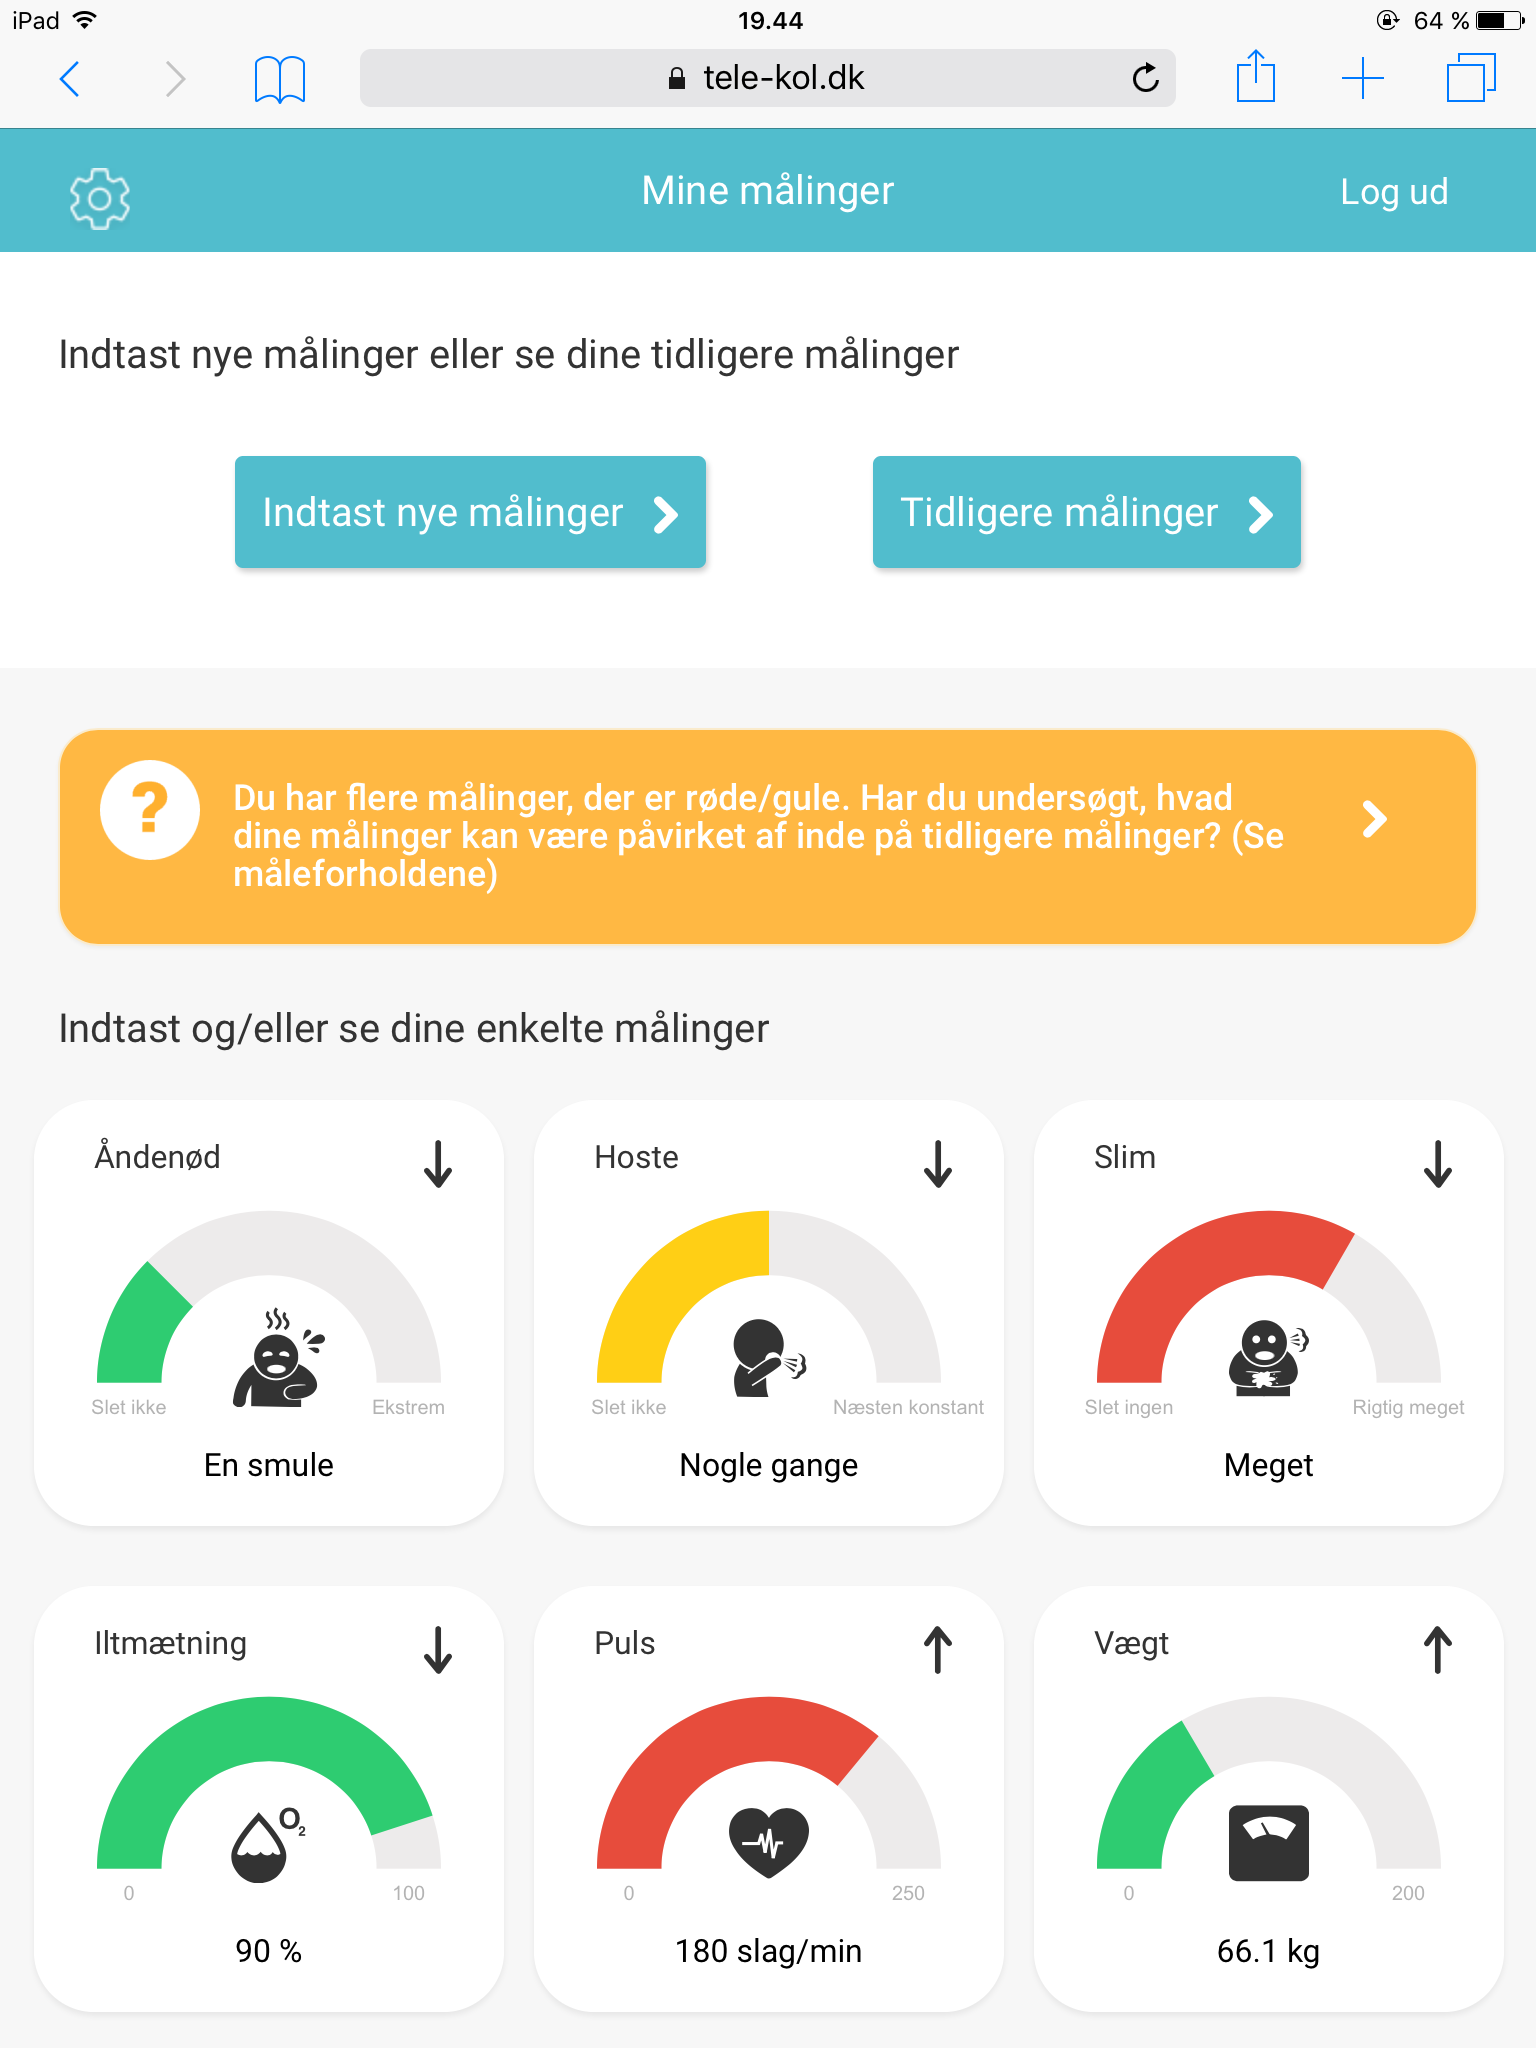
\includegraphics[width=\textwidth]{images/implementation/db.PNG}
    \caption{Shows the dashboard and its design changed made as result of findings from study II.}
    \label{fig:db2nd}
  \end{minipage}
\end{figure}

new interface
 - reflective questions (when they are updated, what are they?)
 - visualisation choice
 - normal areas? what are they based on, individualisation
 

\section{Server-side}


\subsection{Session}



\textbf{Admin Access}

admin features


\subsection{Data Manipulation}
data structure (json, log)
webservice - saveLatestQuestion

 
 
 
\section{Client-side}

\textbf{Get user data}

In order to get each user's data on login, we use ajax from the jquery library. 


\textbf{User interface elements}
one example
 - bootstrap
 
 
\section{Security}
anonymous
https
.htaccess
 - flaws
 - sufficient for trial, .. in operation use of database, programming convenience based on previous experience